%
% teil2.tex -- Beispiel-File für teil2 
%
% (c) 2020 Prof Dr Andreas Müller, Hochschule Rapperswil
%
% !TEX root = ../../buch.tex
% !TEX encoding = UTF-8
%
\section{Nichtlineares Medium
\label{particles:section:nichtlinear}}
\kopfrechts{Nichtlineares Medium}
Entgegen des linearen Mediums, in dem der Proportionalitätsfaktor nicht von der wirkenden Kraft abhängig ist, 
wird dies bei einem nichtlinearen Medium nun zum Problem.
Dies bedeutet also, dass sich das hookesche Gesetz von 
\[
    \Delta l
    = 
    \frac{F}{D}
\]
zu
\[
    \Delta l
    = 
    \frac{F}{D(F)}
\]
abändert. 
Wie dieser Proportionalitätsfaktor genau von der Kraft abhängt, ist je nach Medium unterschiedlich.
Ein Beispiel davon wird im Video~\ref{particles:huygens-optics} von Huygens Optics gezeigt, wobei für $D$ die Formel 
\[
    D(F)
    =
    D_0
    \cdot
    (1 + \alpha |F|^n)
\]
eingesetzt wird.
\begin{figure}
    \centering
    \subfigure[]{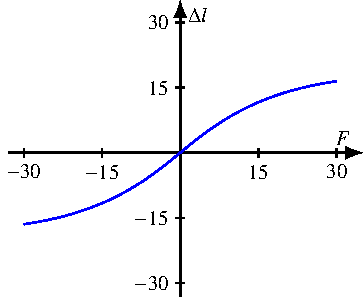
\includegraphics{./papers/particles/figures/out/nichtlineares_medium_deformation.pdf}\label{particles:fig:nichtlin-medium:deform}}\hfill
    \subfigure[]{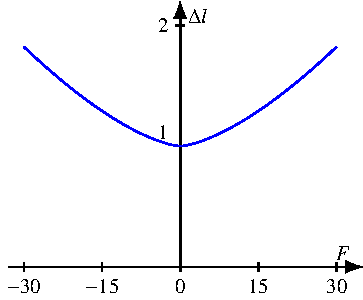
\includegraphics{./papers/particles/figures/out/nichtlineares_medium_elast_modul.pdf}\label{particles:fig:nichtlin-medium:elast-modul}}
    \caption{Deformation~(a) und Elastisches Modul~(b) eines nichtlinearen Mediums mit $D_0 = 1$, $\alpha = 0.005$ und $n = 1.5$.}
\end{figure}

Wiederholen wir nun wieder die Simulation aus Abschnitt~\ref{particles:section:lin-medium:superposition}, so fällt zunächst kein Unterschied auf.
Abbildung~\mytodo{Abbildung mit nichtlinearem Medium und Referenz dazu einfügen} zeigt einen Vergleich der beiden Resultate.
% TODO: Grafik mit gleichem Aufbau wie in "lineares Medium", aber mit nichtlinearem medium (Zwei Lichtwellen)
Damit die Auswirkung der nichtlinearen Effekte erkannt werden können, müssen die Feldstärken scheinbar bedeutend grösser sein.

\subsection{Selbstfokussierung -- Confined Energy}
% TODO: Was für Bedingungen müssen erfüllt sein, damit dies geschieht? 
%       Kann man das überhaupt so einfach klassifizieren?
%       Allenfalls Analogie zu Schwingkreisen herstellen?
Der in Abbildung~\mytodo{Abbildung Anfangszustand} gezeigte Anfangszustand kann durch das Aufeinandertreffen der Wellen im Zentrum besonders grosse Feldstärken hervorrufen.
Wird die Simulation nun abgespielt, so geschieht etwas Unerwartetes: Die Energie im Feld scheint sich im Zentrum zu sammeln.
Die besondere Region inmitten des Simulationsfelds wächst, bis die im Ausgangszustand definierten Wellen entweder gegen den Rand der Simulation verschwinden oder ihre Energie in die Region im Zentrum gesteckt haben.
Dieser Prozess wird in den Abbildungen~\mytodo{Bilder des wachsenden Partikels} veranschaulicht.

Die nächste Phase zeichnet sich durch Oszillieren der symmetrischen Feldanordnung aus. 
Weiter sind einige schwache Wellen zu erkennen, welche die Region der konzentrierten Energie verlassen.
Einige Bilder sind in Abbildung~\mytodo{Bilder des symmetrischen Partikels} gezeigt.

In einer nächsten Phase wird die Symmetrie der Feldanordnung gebrochen, vermutlich da die gespeicherte Energie und so die Grösse der Anordnung zu klein wird.
Aufgrund des Längenelements der ortsdiskreten Simulation sind wohl ab einer gewissen Grösse keine symmetrischen Anordnungen mehr möglich, welche stabil sind.
Die konzentrierte Energie bleibt jedoch einen weiteren Moment bestehen, wie die Abbildung~\mytodo{Bilder asymmetrischer Partikel} zeigt.

In der letzten Phase wird die Energie zu klein, um die Anordnung aufrechtzuerhalten. 
Sie verfällt schliesslich in eine konzentrische, sehr hochfrequente Welle. 
Dessen Wellenlänge ist die in der Simulation kleinstmögliche, sprich zweimal das Längenelement.


Doch was geschieht hier genau? 
\mynote{Analogie zu Schwingkreis herstellen.}
\mynote{Hat das Medium eine Eigenfrequenz? Falls ja, ist diese ausschlaggebend, ob sich die Energie fängt?}
\mynote{Kann man dies als \emph{Soliton} bezeichnen?}

